\section{Gravity}
	For gravity I use the Newtonian equation which provides the magnitude of the force between two bodies. I calculate this during the interact function so the force is calculated between every pair of particles in the universe.
	\begin{equation}
		F = G\frac{m_{1}m_{2}}{r^{2}}
	\end{equation}
	
	Once I have the magnitude I find its direction by finding the angle between the two position vectors and it is applied to each body.
	\begin{figure}[h]
		\centering
		\begin{lstlisting}[language=Scala]
val distance = that.position.distance(position)
val gravForce = (GRAVITATIONAL_CONSTANT * mass * that.mass) / Math.pow(distance, 2)

//Final forces from gravity
List(
  Force(that, gravForce, (this.position - that.position).theta),
  Force(this, gravForce, (that.position - this.position).theta)
)
		\end{lstlisting}
		\caption{The gravity calculations from the Particle class}
		\label{fig:gravCode}
	\end{figure}
	
	\begin{figure}[p]
		\centering
		\begin{subfigure}{0.9\textwidth}
			\centering
			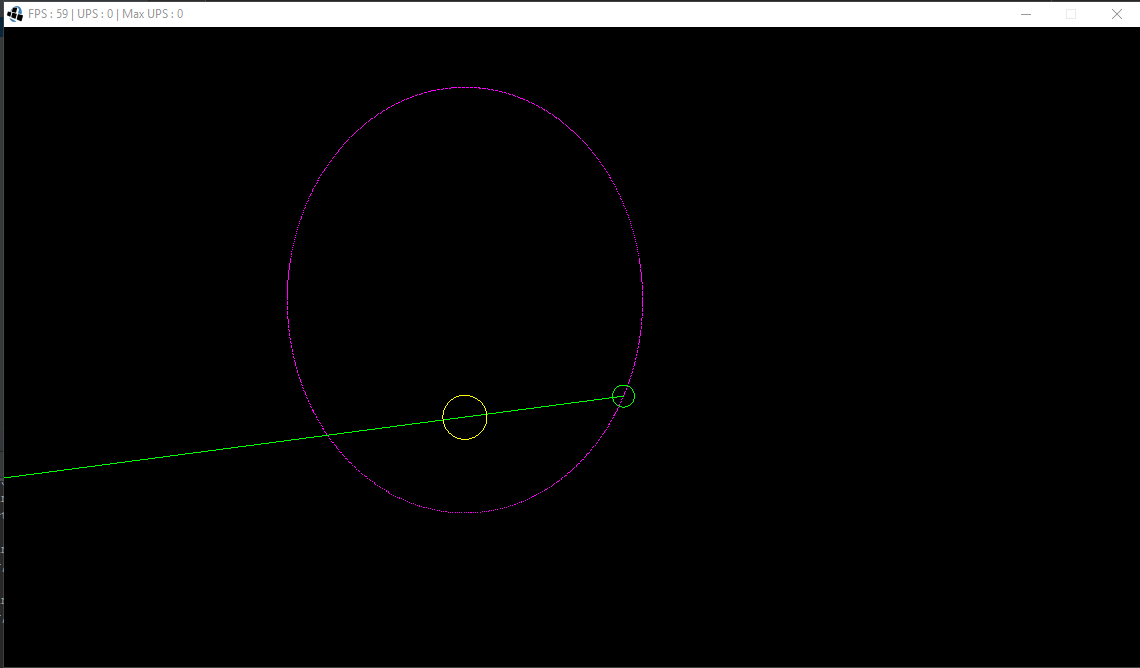
\includegraphics[width=\textwidth]{gravity1}
			\caption{One body in orbit, the orbit is perfectly stable in this case. The green line is the force on the planet.}
			\label{fig:gravExamplesSub1}
			\ref{fig:gravExamplesSub1}
		\end{subfigure}
		\begin{subfigure}{0.9\textwidth}
			\centering
			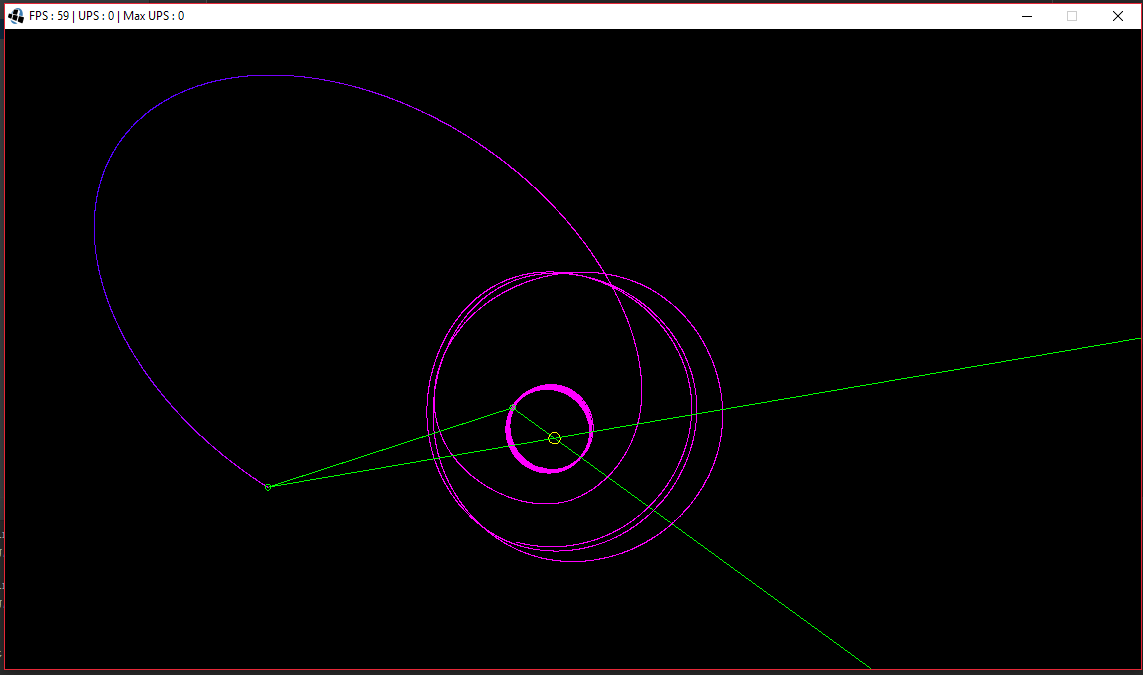
\includegraphics[width=\textwidth]{gravity2}
			\caption{Two bodies in orbit, one is on a more stable orbit whilst the outer one moves more erratically} 
			\label{fig:gravExamplesSub2}
			\ref{fig:gravExamplesSub2}
		\end{subfigure}	
		\caption{Examples of gravity with one and two bodies in orbit around a fixed star}
		\label{fig:gravExamples}
	\end{figure}